\documentclass[aspectratio=169,t]{beamer}
\usepackage[utf8]{inputenc}
\usepackage[T1]{fontenc}
\usepackage[english]{babel}
\usepackage{hyperref}
\usepackage{tikz}

\usepackage{graphicx}
\usepackage{epstopdf}
\usepackage{multirow}

\usepackage{psfrag}
\usepackage{pgfplots}
\usepackage{framed}
\usepackage{xcolor}
\usepackage{booktabs}
\usepackage{caption}
\usepackage{epstopdf}
\usepackage{amsmath}
\usepackage{tabularx}
\usepackage[]{bookmark}
%\usepackage[3D]{movie15}
%\usepackage{media9}
\usepackage[binary-units,abbreviations]{siunitx}
\usepackage[textfont=normalsize, labelfont=normalsize, justification=centering]{subcaption}
\usepackage{marvosym}
\usepackage{calc}
\usepackage{color, colortbl}
\usepackage[]{svg} 
\usepackage[]{trfsigns} 
\usepackage[nomessages]{fp}
\usepackage[]{csquotes}\MakeOuterQuote{"}
\usepackage{tabto}
\selectcolormodel{rgb}

\makeatletter
\def\beamer@calltheme#1#2#3{\def\beamer@themelist{#2}
	\@for\beamer@themename:=\beamer@themelist\do
	{\usepackage[{#1}]{\beamer@themelocation/#3\beamer@themename}}}
\def\usefolder#1{\def\beamer@themelocation{#1}}
\def\beamer@themelocation{}
\usefolder{theme}

\usetikzlibrary{matrix,
	decorations.pathreplacing,
	calc,
	positioning,
	external,
	3d,
	shapes,
	arrows,
	pgfplots.statistics}
\pgfplotsset{compat=1.16}
\tikzstyle{faunode}=[rounded corners, draw=faublue, fill=faublue!10,  align=center, inner sep=0.3cm, line width=0.4mm]
\tikzstyle{fauellipseFixedWidth}=[ellipse, draw=faublue, fill=faublue!10,  align=center, inner sep=0.3cm, line width=0.4mm, minimum width=3cm]
\tikzstyle{fauellipse}=[ellipse, draw=faublue, fill=faublue!10,  align=center, inner sep=0.3cm, line width=0.4mm]
\tikzstyle{fauarrow}=[draw=faublue,->, line width=0.4mm]
\tikzstyle{fauline}=[draw=faublue, line width=0.4mm]


\usepackage[backend=bibtex,sorting=none,doi=true,style=phys]{biblatex}
%\usepackage[]{biblatex}
\bibliography{./references}

% Themes:
%  - fau:          FAU theme
%  - fau-tf:       TechFak FAU theme
%  - fau-tf-lme:   TechFak LME FAU theme
%  - fau-tf-aibe:  TechFak AIBE FAU theme
%
% Options:
%  - image:        Cover image on title page
%  - plain:        Plain title page
%  - longtitle:    Title page layout for long title
% \usetheme[longtitle]{fau-tf-lme}
\usetheme[longtitle]{fau-tf-aibe}

% END of THEME SETTINGS
% --------------------------------------------------------------------------------------------------------------------------------------------------------------------------

\sisetup{
exponent-product =\ensuremath{{\,\cdot\,}}
}

% Enable semi-transparent animation preview
\setbeamercovered{transparent}
\setbeamertemplate{blocks}[rounded]
\captionsetup{labelformat=empty,labelsep=none, labelfont=normalsize, justification=centering}


\newcommand\Wider[2][1.0cm]{%
\makebox[\linewidth][c]{%
  \begin{minipage}{\dimexpr\textwidth+#1\relax}
  \raggedright#2
  \end{minipage}%
  }%
}


\let\origitem\item
\renewcommand{\item}{\normalfont\origitem}
\newcommand{\bluefat}[1]{\textcolor{faublue}{\textbf{#1}}}
\newcommand{\bolditem}{\normalfont\origitem\bfseries}
\newcommand{\question}{{\bf Question: }}
\newcommand{\answer}{{\bf Answer: }}
\newcommand{\myExample}{{\bf Example }}
\newcommand{\real}{\mbox{${\mathbb R}$}}
\definecolor{defColor}{rgb}{0.8,0.87,0.97}
\definecolor{defColorT}{rgb}{0,0,0}
\definecolor{defColorF}{rgb}{1,1,1}
\newenvironment{myDefinition}{%
	\def\FrameCommand{\fboxsep=\FrameSep{} \fcolorbox{defColorF}{defColor}}%
	\color{defColorT}\MakeFramed{\FrameRestore{}}}%
{\endMakeFramed}

% Title page
\title[Medical Engineering II]{Medical Engineering - Imaging Systems}

\author{Prof.\ Dr. Bernhard Kainz \and Prof.\ Dr. Florian Knoll}
\date{SS 2024}
\institute{IDEA Lab and Computational Imaging Lab at Dept. AIBE}

\newcommand{\password}{\texttt{mt2\_ss22}}


\AtBeginSection[]{
	{
		\setbeamertemplate{footline}{}
		\begin{frame}[noframenumbering]{\insertsubtitle}
			 \tableofcontents[currentsection]
		\end{frame} 
	}
}
\AtBeginSubsection[]{
	{

		\setbeamertemplate{footline}{}
		\begin{frame}[noframenumbering]{\insertsubtitle}
			 \tableofcontents[currentsection, currentsubsection]
		\end{frame} 
	}
}


\newcommand{\TODO}[1]{\textcolor{red}{[\textbf{TODO}: #1]}}
\newcommand{\specialcell}[2][l]{\begin{tabular}[#1]{@{}c@{}}#2\end{tabular}}
\newcommand{\cont}{(cont.)}


\usepackage{animate}
\usepackage{latexsym}
\usepackage{bm}
\usepackage{import}
\usepackage{transparent}

\subtitle{Ultra Sound}

\AtBeginSection[]{
    {
        \setbeamertemplate{footline}{}
        \begin{frame}[noframenumbering]{\insertsubtitle}
            \large \tableofcontents[currentsection]
        \end{frame} 
    }
}
\AtBeginSubsection[]{
    {

        \setbeamertemplate{footline}{}
        \begin{frame}[noframenumbering]{\insertsubtitle}
            \large \tableofcontents[currentsection, currentsubsection]
        \end{frame} 
    }
}

\begin{document}

\frame[plain,c]{\titlepage} % plain-Option deaktiviert Kopf- und Fusszeile

%%%%%%%%%%%%%%%%%%%%%%%%%%%%%%%%%%%%%%%%%%%%%%%%%%%%%%%%%%%%
%%%%%%%%%%%%%%%%%%%%%%%%%%%%%%%%%%%%%%%%%%%%%%%%%%%%%%%%%%%%
\section{Ultrasound Applications}
%%%%%%%%%%%%%%%%%%%%%%%%%%%%%%%%%%%%%%%%%%%%%%%%%%%%%%%%%%%%
%%%%%%%%%%%%%%%%%%%%%%%%%%%%%%%%%%%%%%%%%%%%%%%%%%%%%%%%%%%%


%%%%%%%%%%%%%%%%%%%%%%%%%%%%%%%%%%%%%%%%%%%%%%%%%%%%%%%%%%%%
\begin{frame}{Ultrasound Applications: SONAR}
    \begin{figure}
        \centering
        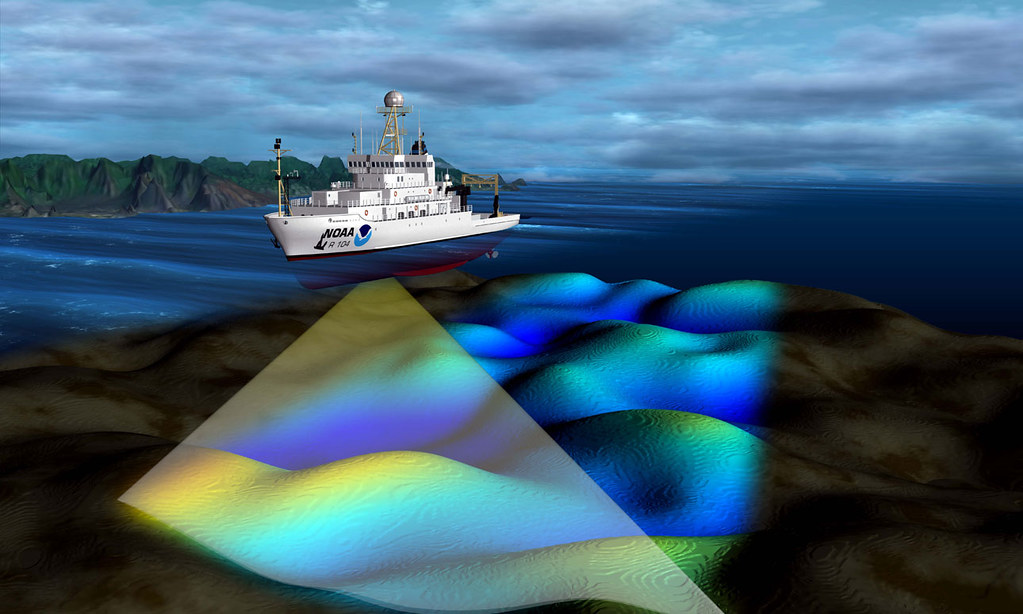
\includegraphics[height=0.8\textheight]{images/sonar.jpg}\\
        {\scriptsize Source: National Ocean Service}
        %Creative Commons by Attribution
    \end{figure}
\end{frame}


%%%%%%%%%%%%%%%%%%%%%%%%%%%%%%%%%%%%%%%%%%%%%%%%%%%%%%%%%%%%
\begin{frame}{Ultrasound Applications: Echolocation}
    \begin{figure}
        \centering
        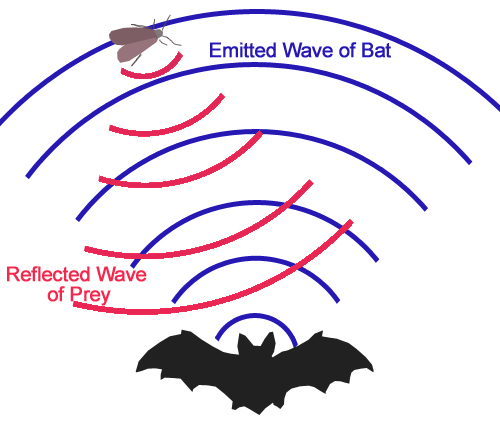
\includegraphics[height=0.7\textheight]{images/Bat_echolocation.jpg}\\
    \end{figure}
    \begin{flushright}
        \tiny
        Source: By Shung \url{https://commons.wikimedia.org/w/index.php?curid=11999649}
    \end{flushright}
\end{frame}


%%%%%%%%%%%%%%%%%%%%%%%%%%%%%%%%%%%%%%%%%%%%%%%%%%%%%%%%%%%%
%\begin{frame}{Ultrasound Applications: Medical}
%\begin{figure}
%\centering
%\includegraphics[width=.66\linewidth]{images/us_east_germany_1990.jpg}\\
%{ Ultrasound examination of pregnant woman (1990). Source: \href{http://www.bild.bundesarchiv.de/archives/barchpic/search/_1389292888/}{Bundesarchiv}.}
%\end{figure}
%\end{frame}

\begin{frame}{Ultrasound Applications: Medical}
    \begin{figure}
        \centering
        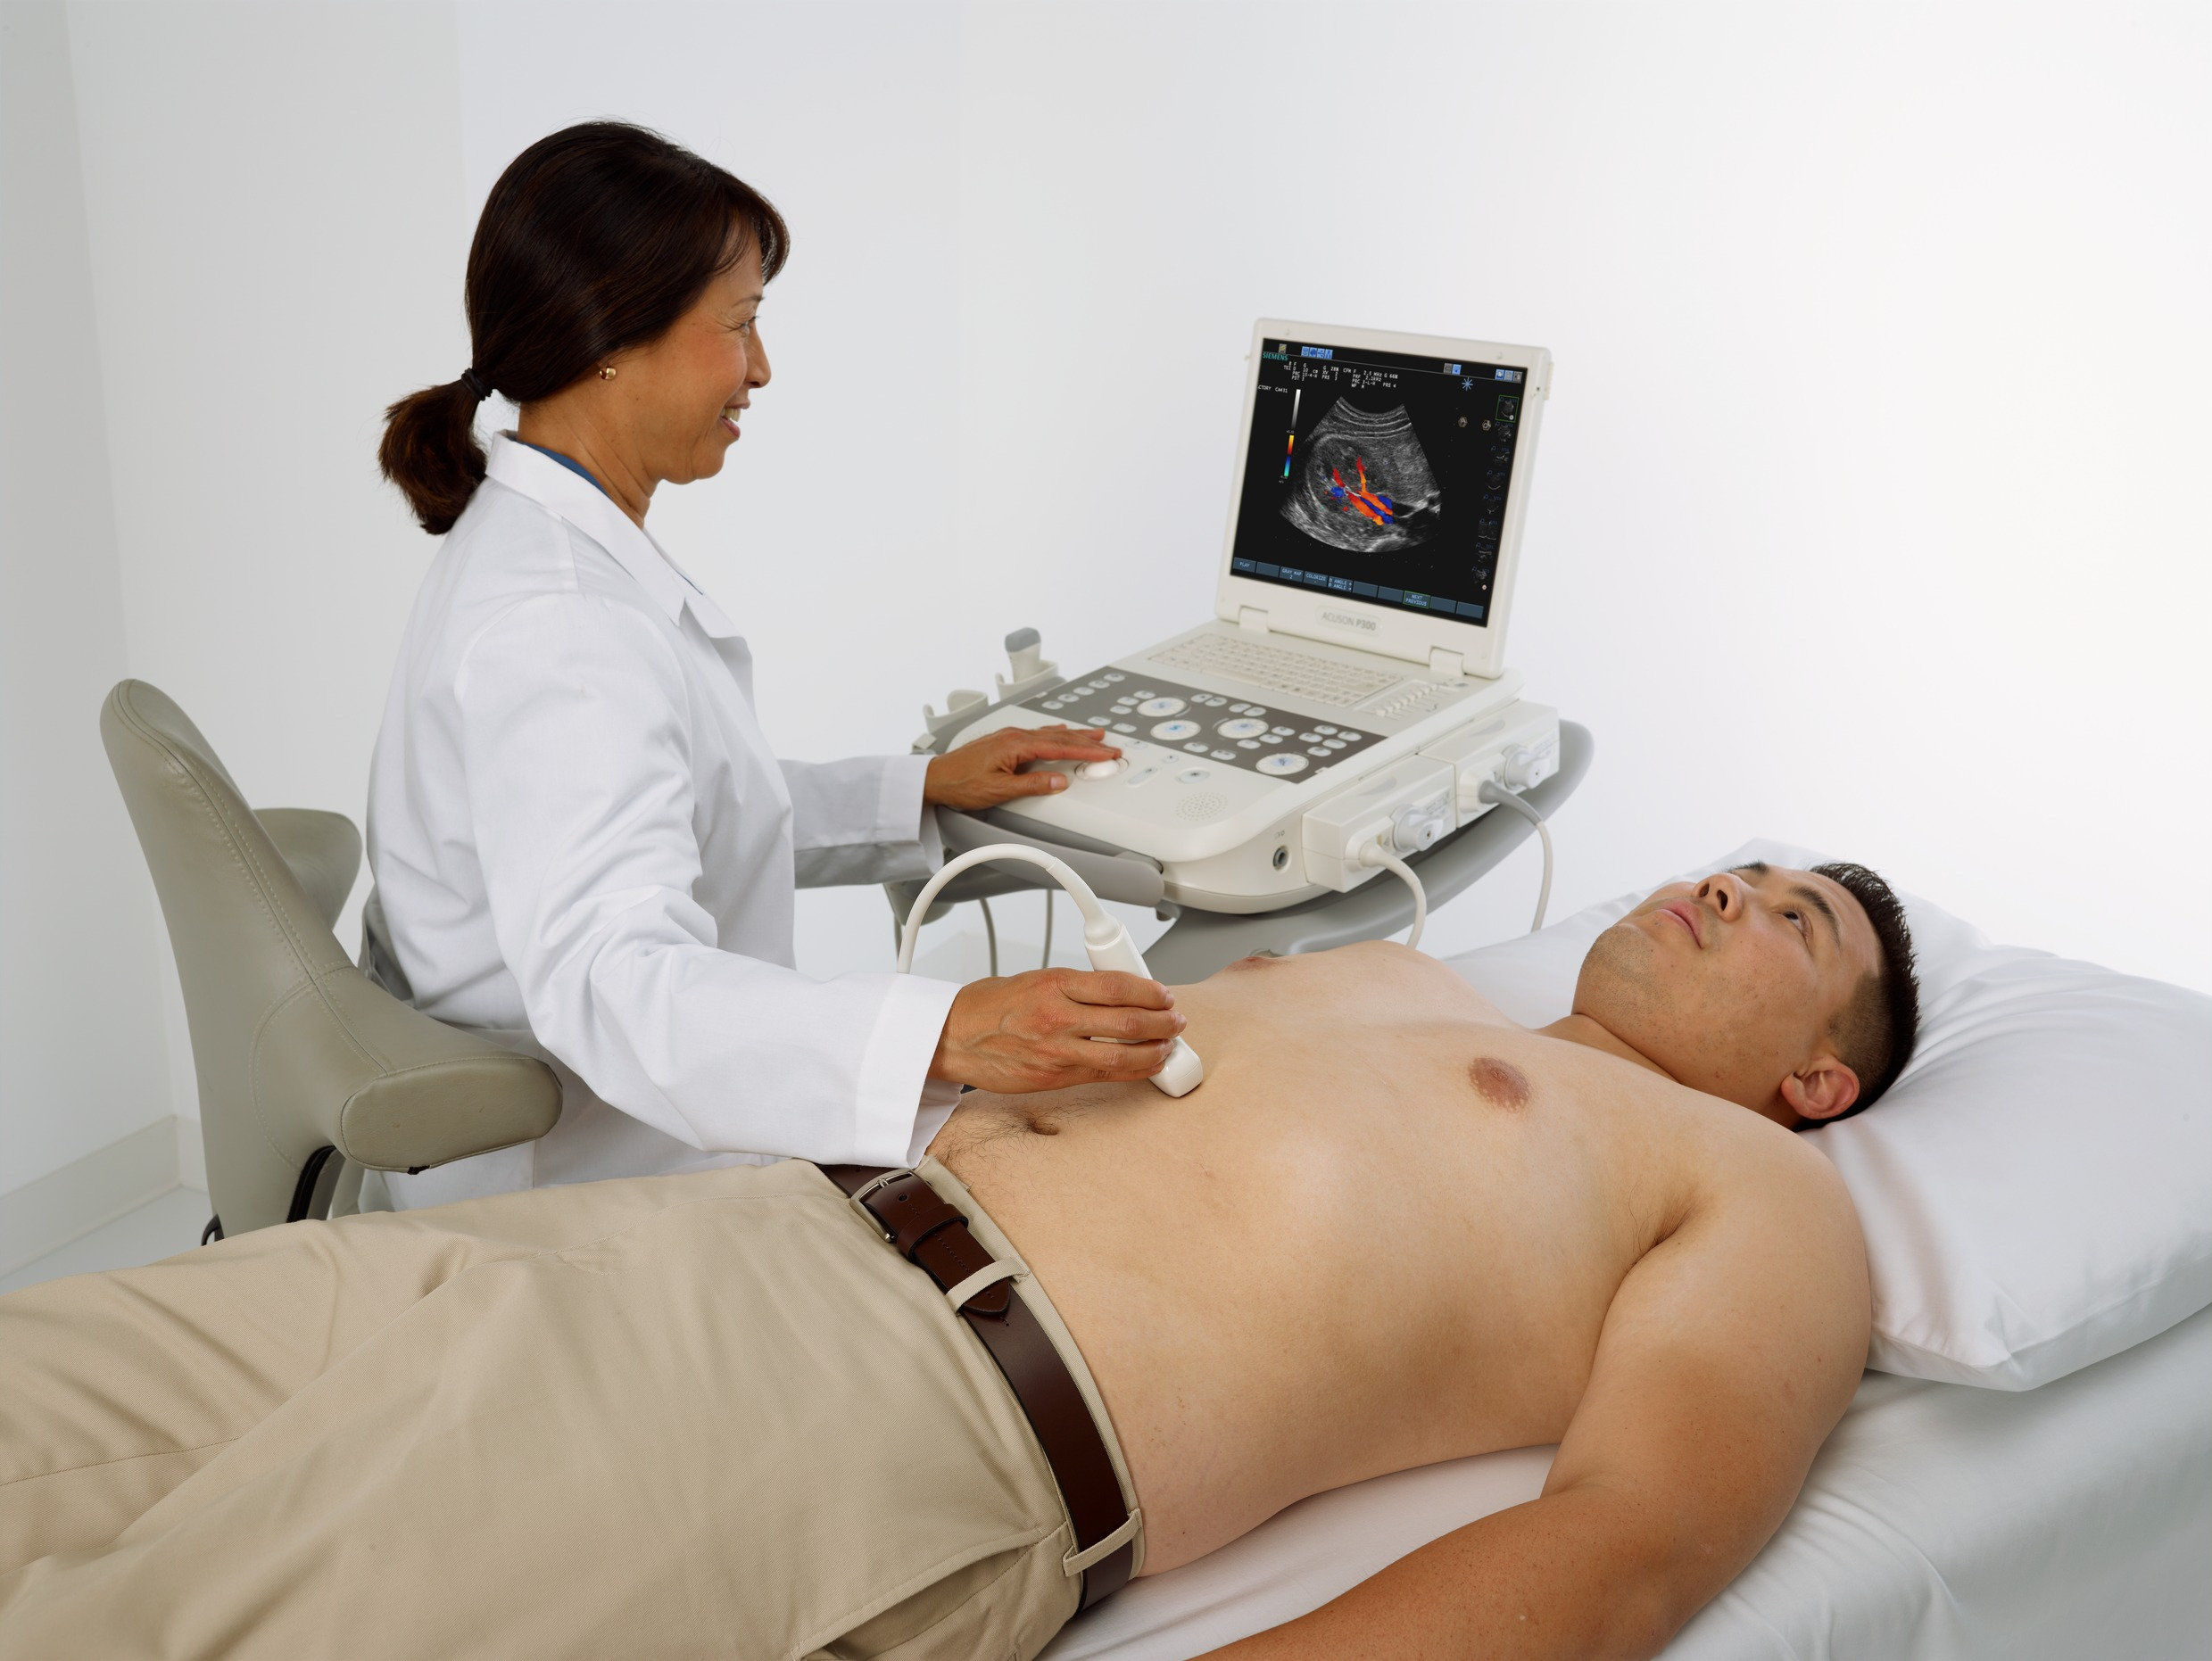
\includegraphics[height=0.8\textheight]{images/SH_US_35403_12.jpg}\\
        %{ Ultrasound examination of pregnant woman (1990). Source: \href{http://www.bild.bundesarchiv.de/archives/barchpic/search/_1389292888/}{Bundesarchiv}.}
    \end{figure}
\end{frame}

%%%%%%%%%%%%%%%%%%%%%%%%%%%%%%%%%%%%%%%%%%%%%%%%%%%%%%%%%%%%
\begin{frame}{Ultrasound Applications: Medical \cont}
    \begin{figure}
        \centering
        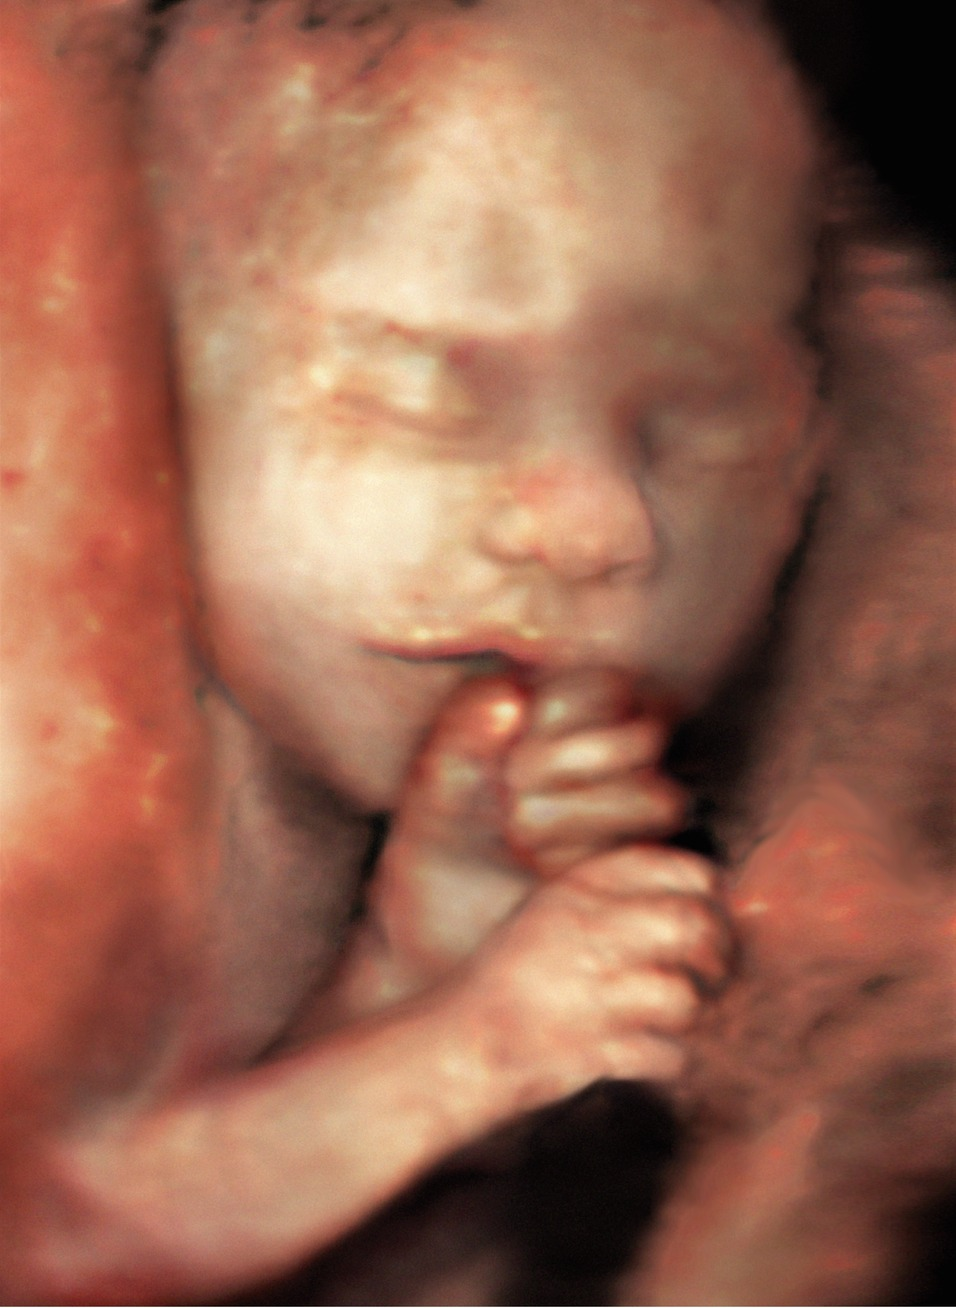
\includegraphics[height=0.8\textheight]{images/SH_US_34572_12.jpg}\\
        \caption{3D Ultrasound of fetuses. Source:~\cite{neumann18}}
    \end{figure}
\end{frame}


%%%%%%%%%%%%%%%%%%%%%%%%%%%%%%%%%%%%%%%%%%%%%%%%%%%%%%%%%%%%%

\begin{frame}{Ultrasound Applications: Medical \cont}
    \begin{figure}
        \centering
        \href{https://upload.wikimedia.org/wikipedia/commons/transcoded/5/56/Uotw78.webm/Uotw78.webm.360p.vp9.webm}{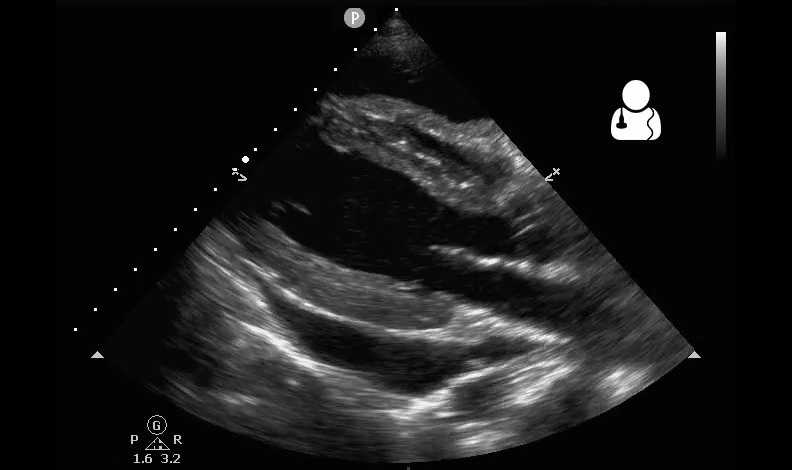
\includegraphics[height=0.8\textheight]{images/uotw78.jpg}}\\
        \caption{Ultrasound image of a beating heart (click for video).}
        %Creative Common License!
    \end{figure}
    \begin{flushright}
        \tiny
        Source: \url{ultrasoundoftheweek.com}
    \end{flushright}
\end{frame}


%\begin{frame}{Ultrasound Applications: Medical \cont}
%\begin{figure}
%\centering
%\includegraphics[width=.47\linewidth]{images/SH_US_34608_12.jpg} \enspace
%\includegraphics[width=.451\linewidth]{images/tte_2d_example.jpg}\\
%{ Transthoracic echocardiography. Source: \url{http://echocardiographer.org/}}
%\end{figure}
%\end{frame}


%%%%%%%%%%%%%%%%%%%%%%%%%%%%%%%%%%%%%%%%%%%%%%%%%%%%%%%%%%%%%
%\begin{frame}{Ultrasound Applications: Medical \cont}
%\begin{figure}
%\centering
%\includegraphics[width=.4\linewidth]{images/tee_illustration.jpg}\\
%{ Transesophageal echocardiography. Source: \url{http://echocardiographer.org/}}
%\end{figure}
%\end{frame}


%%%%%%%%%%%%%%%%%%%%%%%%%%%%%%%%%%%%%%%%%%%%%%%%%%%%%%%%%%%%
\begin{frame}[c]{Ultrasound Applications: Medical \cont}
    \structure{Applications of ultrasound in medicine}
    \begin{itemize}
        \item Pregnancy
        \item Gynecology
        \item Gastrointestinal tract
        \item Heart
        \item Blood vessels (stenosis, aneurysms)
        \item Blood flow
        \item \dots
    \end{itemize}

\end{frame}


%%%%%%%%%%%%%%%%%%%%%%%%%%%%%%%%%%%%%%%%%%%%%%%%%%%%%%%%%%%%
%%%%%%%%%%%%%%%%%%%%%%%%%%%%%%%%%%%%%%%%%%%%%%%%%%%%%%%%%%%%
\section{Ultrasound in Medicine}
%%%%%%%%%%%%%%%%%%%%%%%%%%%%%%%%%%%%%%%%%%%%%%%%%%%%%%%%%%%%
%%%%%%%%%%%%%%%%%%%%%%%%%%%%%%%%%%%%%%%%%%%%%%%%%%%%%%%%%%%%


%%%%%%%%%%%%%%%%%%%%%%%%%%%%%%%%%%%%%%%%%%%%%%%%%%%%%%%%%%%%
\begin{frame}[c]{Ultrasound Imaging}
    \structure{Ultrasound (US) imaging} (or \structure{ultrasonography})
    \begin{itemize}
        \item A medical imaging technique that uses high frequency sound waves and their echoes
        \item[$\rightarrow$] similar to echolocation (bats, whales, dolphins) and SONAR (submarines)
    \end{itemize}

    %\vspace{.5cm}
    %\structure{In a nutshell}
    %\begin{itemize}
    %\item US pulses are transmitted into the patient
    %\item The reflection (echo) of pulsed ultrasound waves is measured
    %\item 
    %\end{itemize}

\end{frame}


%%%%%%%%%%%%%%%%%%%%%%%%%%%%%%%%%%%%%%%%%%%%%%%%%%%%%%%%%%%%
\begin{frame}{Ultrasound Imaging \cont}

    \structure{Acoustic spectrum}
    \vspace{.3cm}
    \begin{center}
        \begin{tabular}{c|c|c|}
            \hline
            {}                     & {Frequencies $f$}  & {Examples}         \\\hline\hline
            \textbf{Infrasound}    & 0 \dots 16 Hz      & Seismic waves      \\\hline
            \textbf{Audible sound} & 16 Hz \dots 20 kHz & \specialcell{Music \\Human speech}\\\hline
            \textbf{Ultrasound}    & 20 kHz and up      & \specialcell{Bats  \\Dolphins\\SONAR\\Acoustic microscopy\\Medical Imaging}\\\hline
        \end{tabular}
    \end{center}

    \vspace{.6cm}
    $\rightarrow$ \structure{Medical} ultrasound: $f \approx 1$ MHz $\dots 40$ MHz
\end{frame}


%%%%%%%%%%%%%%%%%%%%%%%%%%%%%%%%%%%%%%%%%%%%%%%%%%%%%%%%%%%%
\begin{frame}[c]{Historical Remarks}
    \structure{From discovery of underlying physical principles to first clinical scanner}
    \vspace{.1cm}

    \begin{columns}[t, onlytextwidth]
        \begin{column}{0.05\textwidth}
        \end{column}\begin{column}{0.9\textwidth}
            \begin{itemize}
                \item<2->[\bluefat{1880:}] Discovery of \structure{piezoelectic} effect
                \item<3->[\bluefat{1920:}] Ultrasound-based distance measurement in water (SONAR)
                \item<4->[\bluefat{1933:}] Therapeutic use of ultrasound
                \item<5->[\bluefat{1952:}] First 2D pulse echo image
                \item<6->[\bluefat{1953:}] Breast imaging using ultrasound
                \item<7->[\bluefat{1957:}] Echocardiography using ultrasound motion mode (M-mode)
                \item<8->[\bluefat{1957:}] Doppler imaging
                \item<9->[\bluefat{1958:}] First ultrasound scanner in \structure{clinical} use
            \end{itemize}
        \end{column}
    \end{columns}

\end{frame}


%%%%%%%%%%%%%%%%%%%%%%%%%%%%%%%%%%%%%%%%%%%%%%%%%%%%%%%%%%%%
%\begin{frame}{Historical Remarks \cont}
%\begin{figure}
%\centering
%\includegraphics[width=.78\linewidth]{images/first_scanner_1957.png}\\
%{ Medicine section in LIFE Magazine (1954).}
%\end{figure}

%\end{frame}



%%%%%%%%%%%%%%%%%%%%%%%%%%%%%%%%%%%%%%%%%%%%%%%%%%%%%%%%%%%%%
%\begin{frame}{Historical Remarks \cont}
%\begin{columns}[b]
%\column{.45\textwidth}
%\begin{figure}
%\centering
%\includegraphics[width=.8\columnwidth]{images/us_toshiba_1976.jpg}\\
%{ Toshiba SSL-35H (1976).}
%\end{figure}

%\column{.45\textwidth}
%\begin{figure}
%\centering
%\includegraphics[width=.73\columnwidth]{images/portable_us_siemens_2012.jpg}\\
%{ Siemens Acuson P300 portable (2012).}
%\end{figure}
%\end{columns}
%\end{frame}


%%%%%%%%%%%%%%%%%%%%%%%%%%%%%%%%%%%%%%%%%%%%%%%%%%%%%%%%%%%%
%%%%%%%%%%%%%%%%%%%%%%%%%%%%%%%%%%%%%%%%%%%%%%%%%%%%%%%%%%%%
\section{Physics of Sound Waves}
%%%%%%%%%%%%%%%%%%%%%%%%%%%%%%%%%%%%%%%%%%%%%%%%%%%%%%%%%%%%
%%%%%%%%%%%%%%%%%%%%%%%%%%%%%%%%%%%%%%%%%%%%%%%%%%%%%%%%%%%%


%%%%%%%%%%%%%%%%%%%%%%%%%%%%%%%%%%%%%%%%%%%%%%%%%%%%%%%%%%%%
\begin{frame}[c]{Sound Waves}

    \bluefat{Waves}
    \begin{itemize}
        \setlength\itemsep{0.3cm}
        \item Spatially propagating, periodically repeating processes
        \item Distinction based on \structure{direction of propagation}
              \begin{itemize}
                  \item Transverse waves
                  \item Longitudinal waves
              \end{itemize}
    \end{itemize}
    \vspace{1cm}

    \bluefat{Sound Waves}

    \begin{itemize}
        \item \structure{Sound waves} are \structure{longitudinal} waves
        \item Caused by \structure{local periodic compression} of matter
        \item In liquids and gases: only longitudinal waves possible
    \end{itemize}

\end{frame}


%%%%%%%%%%%%%%%%%%%%%%%%%%%%%%%%%%%%%%%%%%%%%%%%%%%%%%%%%%%%
\begin{frame}{Sound Waves \cont}
    \begin{columns}[c, onlytextwidth]
        \begin{column}{0.6\textwidth}
            Sound waves can be \structure{characterized} by

            \vspace{.5cm}
            \begin{itemize}
                \setlength\itemsep{0.3cm}
                \item Frequency $f$ (Hz)
                      \begin{itemize}
                          \item Oscillation count per second
                      \end{itemize}
                \item Sound velocity $v$ (m\,s$^{-1}$)
                      \begin{itemize}
                          \item Independent of $f$
                          \item Varies with material properties (e.g.~elasticity, density)
                      \end{itemize}
                \item Wavelength $\lambda$ (m)\\
                      \begin{itemize}
                          \item Distance between two oscillation maxima
                      \end{itemize}
                \item Intensity $J$ (W\,m$^{-2}$)\\
                      \begin{itemize}
                          \item Acoustic power density
                      \end{itemize}
            \end{itemize}
        \end{column}\begin{column}{0.5\textwidth}
            \centering{}
            \structure{Fundamental} wave equation:
            \begin{equation*}
                \lambda = c / f
            \end{equation*}
        \end{column}
    \end{columns}
\end{frame}


%%%%%%%%%%%%%%%%%%%%%%%%%%%%%%%%%%%%%%%%%%%%%%%%%%%%%%%%%%%%
\begin{frame}{Sound Waves \cont}

    \begin{figure}
        \def\svgwidth{.6\columnwidth}
        \import{images/}{longitudinal_wave_3d.pdf_tex}
    \end{figure}

\end{frame}


%%%%%%%%%%%%%%%%%%%%%%%%%%%%%%%%%%%%%%%%%%%%%%%%%%%%%%%%%%%%
\begin{frame}{Sound Waves \cont}

    \vspace{.4cm}
    \begin{figure}
        \def\svgwidth{.5\columnwidth}
        \import{images/}{longitudinal_wave.pdf_tex}\\
        { Mass-spring model of longitudinal wave}
    \end{figure}

    $\rightarrow$ \structure{Sound velocity} $v = {\mathsf{d} s}/{\mathsf{d} t}$

\end{frame}


%%%%%%%%%%%%%%%%%%%%%%%%%%%%%%%%%%%%%%%%%%%%%%%%%%%%%%%%%%%%%
%\begin{frame}{Sound Wave Characterization \cont}
%
%Acoustic pressure for \structure{planar wave} (travelling in z-direction)
%$$\frac{\partial^2 p(z,t)}{\partial z^2} = \frac{1}{c^2} \cdot \frac{\partial^2 p(z,t)}{\partial t^2}$$
%
%\vspace{1cm}
%Example \structure{solution}
%$$p(z,t) = \cos k(z-tc)$$
%%
%{
%\begin{eqnarray*}
%k&:& \text{Wave number } (k = 2\pi / \lambda)
%\end{eqnarray*}}
%
%\structure{Cyclic frequency} $f$ of the above solution and \structure{relation to wave length} $\lambda$
%$$f = \frac{kc}{2\pi} \Rightarrow f = \frac{c}{\lambda}$$
%
%\end{frame}


%%%%%%%%%%%%%%%%%%%%%%%%%%%%%%%%%%%%%%%%%%%%%%%%%%%%%%%%%%%%
\begin{frame}{Sound Waves \cont}

    \structure{Acoustic impedance} $Z$ (g\,cm$^{-2}$\,s$^{-1}$)

    \vspace{1cm}
    $Z$ of a medium is determined by its \structure{material properties}
    \vspace{.2cm}
    $$Z = \sqrt{E \cdot D}$$

    {
            \begin{eqnarray*}
                Z&:& \text{Acoustic impedance}\\
                E&:& \text{Tensile modulus (elasticity)}\\
                D&:& \text{Density of medium}
            \end{eqnarray*}}

    %{$\rightarrow$ Sound travels through materials under the influence of sound pressure.
    %Because molecules of a solid are bound elastically to one another, the excess pressure results in a wave propagating through the solid.}

\end{frame}


%%%%%%%%%%%%%%%%%%%%%%%%%%%%%%%%%%%%%%%%%%%%%%%%%%%%%%%%%%%%
\begin{frame}{Sound Waves \cont}

    \structure{Sound velocity in, and impedance of various biological materials}

    \vspace{0.6cm}
    \begin{center}
        \begin{tabular}{lrr}
            \toprule{}
            \textbf{Medium} & $v$ [m/s] & $Z$ [g\,cm$^{-2}$\,s$^{-1}$] \\
            \midrule{}{Air} & 331       & 43                           \\
            {Fat}           & 1470      & 1.42 $\cdot$ 10$^5$          \\
            {Water}         & 1492      & 1.48 $\cdot$ 10$^5$          \\
            {Brain tissue}  & 1530      & 1.56 $\cdot$ 10$^5$          \\
            {Muscles}       & 1568      & 1.63 $\cdot$ 10$^5$          \\
            {Bones}         & 3600      & 6.12 $\cdot$ 10$^5$          \\
            \bottomrule{}
        \end{tabular}
    \end{center}

\end{frame}


%%%%%%%%%%%%%%%%%%%%%%%%%%%%%%%%%%%%%%%%%%%%%%%%%%%%%%%%%%%%%
%\begin{frame}{Sound Waves \cont}
%
%\structure{Velocity, impedance and density of various biological materials}
%
%\vspace{0.6cm}
%\begin{center}
%\begin{tabular}{|r||r|r|r|}
%\hline
%\textbf{Medium} & $c$ [m/s] & $Z$ [g\,cm$^{-2}$\,s$^{-1}$] & $D$ [g\,cm$^{-3}$]\\\hline\hline
%{Air} & 331 & 43 & 0.013 \\\hline
%{Fat} & 1470 & 1.42 $\cdot$ 10$^5$ & 0.97 \\\hline
%{Water} & 1492 & 1.48 $\cdot$ 10$^5$ & 0.9982 \\\hline
%{Brain tissue} & 1530 & 1.56 $\cdot$ 10$^5$ & 1.02 \\\hline
%{Muscles} & 1568 & 1.63 $\cdot$ 10$^5$ & 1.04 \\\hline
%{Bones} & 3600 & 6.12 $\cdot$ 10$^5$ & 1.7 \\\hline
%\end{tabular}
%\end{center}
%
%\end{frame}


%%%%%%%%%%%%%%%%%%%%%%%%%%%%%%%%%%%%%%%%%%%%%%%%%%%%%%%%%%%%
\begin{frame}{Characteristics at Boundaries}

    \begin{columns}[T]

        \column{0.5\linewidth}
        At boundaries between two media, sound waves \dots
        \begin{itemize}
            \item \dots are \structure{partially reflected}\\
                  \hspace{1cm}{ $\rightarrow$ Reflection coefficient}
                  $$R = \frac{J_r}{J_0} = \left(\frac{Z_2-Z_1}{Z_2+Z_1}\right)^2$$
                  \vspace{.1cm}
            \item \dots and \structure{partially transmitted}\\
                  \hspace{1cm}{ $\rightarrow$ Transmission coefficient}
                  $$T = \frac{J_t}{J_0} = \frac{4\cdot Z_1 \cdot Z_2}{\left(Z_1+Z_2\right)^2}$$
            \item[$\Rightarrow$] Holds for perpendicular incidence
        \end{itemize}
        \vspace{.5cm}

        \column{0.4\linewidth}
        \vspace{-.5cm}
        \begin{figure}
            \def\svgwidth{.85\columnwidth}
            \import{images/}{reflection_transmission_perpendicular.pdf_tex}
        \end{figure}
        \vspace{-0.4cm}
        { $\rightarrow$ $J_0, J_r, J_t$: Acoustic intensities [W\,m$^{-2}$]}
    \end{columns}

\end{frame}


%%%%%%%%%%%%%%%%%%%%%%%%%%%%%%%%%%%%%%%%%%%%%%%%%%%%%%%%%%%%
\begin{frame}{Characteristics at Boundaries \cont}
    \structure{Reflectivity at boundaries between various materials}
    \vspace{0.6cm}
    \begin{center}
        \begin{tabular}{llr}
            \toprule{}
            \textbf{Material 1}                  & \textbf{Material 2} & \textbf{Reflected portion} \\
            \rowcolor{faublue!10}\midrule{}Brain & Skull bone          & 43.5\,\%                   \\
            Fat                                  & Muscle              & 1\,\%                      \\
            \rowcolor{faublue!10}Fat             & Kidney              & 0.6\,\%                    \\
            Muscle                               & Blood               & 0.1\,\%                    \\
            \rowcolor{faublue!10}Soft tissue     & Water               & 0.25\,\%                   \\
            Soft tissue                          & Air                 & 99.9\,\%                   \\
            \bottomrule{}
        \end{tabular}
    \end{center}

\end{frame}


%%%%%%%%%%%%%%%%%%%%%%%%%%%%%%%%%%%%%%%%%%%%%%%%%%%%%%%%%%%%
\begin{frame}{Characteristics at Boundaries \cont}
    Reflection of sound waves at smooth surfaces (\structure{angles} $\alpha_1, \alpha_2$)
    \begin{figure}
        \def\svgwidth{.5\linewidth}
        \import{images/}{reflection_transmission.pdf_tex}
    \end{figure}
    $$\alpha_1 = \alpha_2$$

\end{frame}


%%%%%%%%%%%%%%%%%%%%%%%%%%%%%%%%%%%%%%%%%%%%%%%%%%%%%%%%%%%%
\begin{frame}{Characteristics at Boundaries \cont}
    Diffuse reflection at \structure{rough boundaries}
    \begin{figure}
        \def\svgwidth{.5\linewidth}
        \import{images/}{reflection_diffuse.pdf_tex}
    \end{figure}
    { $\rightarrow$ \structure{Width} of reflection cone \structure{increases} with \structure{decreasing $\lambda$} and \structure{increasing roughness}}

\end{frame}


%%%%%%%%%%%%%%%%%%%%%%%%%%%%%%%%%%%%%%%%%%%%%%%%%%%%%%%%%%%%
\begin{frame}{Characteristics at Boundaries \cont}

    \begin{columns}[T]
        \column{0.65\linewidth}
        Small inhomogeneities (size: $a$) in the material cause \structure{scattering} of the waves.

        \vspace{.5cm}
        \begin{itemize}
            \item $a \gg \lambda$: \structure{Geometric} range (high scattering)\\\hspace{2.5cm}{ $\rightarrow$ Vessels}\vspace{.5cm}
            \item $a \approx \lambda$: \structure{Stochastic} range (medium scattering)\\\hspace{2.5cm}{ $\rightarrow$ Liver}\vspace{.5cm}
            \item $a \ll \lambda$: \structure{Rayleigh} range (low scattering)\\\hspace{2.5cm}{ $\rightarrow$ Blood}
        \end{itemize}

        \column{0.25\linewidth}
        \begin{figure}
            \def\svgwidth{0.9\columnwidth}
            \import{images/}{inhomogeneities.pdf_tex}
        \end{figure}
    \end{columns}

\end{frame}


%%%%%%%%%%%%%%%%%%%%%%%%%%%%%%%%%%%%%%%%%%%%%%%%%%%%%%%%%%%%
\begin{frame}[c]{Characteristics at Boundaries \cont}
    \structure{Reflection}
    \begin{itemize}
        \item Reflection defines borders in ultrasound images
        \item Large portions of the incident intensity can be reflected\\
              \begin{itemize}
                  \item[$\rightarrow$] especially at borders of materials with large difference in impedance
              \end{itemize}
    \end{itemize}
    \vspace{.5cm}
    \structure{Scattering} \dots
    \begin{itemize}
        \item \dots adds to reflective response
        \item \dots generates speckle noise
              \begin{itemize}
                  \item[$\rightarrow$] especially for inhomogeneities with $a \approx \lambda$ (geometric range)
              \end{itemize}
    \end{itemize}
    \vspace{.5cm}

\end{frame}


%%%%%%%%%%%%%%%%%%%%%%%%%%%%%%%%%%%%%%%%%%%%%%%%%%%%%%%%%%%%
\begin{frame}{Attenuation}
    \structure{Exponential law} of attenuation

    \begin{equation}
        J(x) = J_0\cdot\exp{(-\mu \cdot x})
    \end{equation}

    \begin{itemize}
        \item[$\Rightarrow$] Acoustic intensity $J$ \structure{decreases} with \structure{increasing penetration depth} ($x$)
    \end{itemize}

    \vspace{1cm}
    \structure{Attenuation coefficient} $\mu$ [dB]
    \begin{itemize}
        \item Attenuation that occurs with each cm the sound wave travels in a medium
        \item Depends on material (tissue type) and ultrasound frequency $f$
        \item Consists of absorption $\mu_a$ and scattering $\mu_s$ part: $\mu = \mu_a + \mu_s$
        \item Absorption leads to heating of tissue
    \end{itemize}
\end{frame}


%%%%%%%%%%%%%%%%%%%%%%%%%%%%%%%%%%%%%%%%%%%%%%%%%%%%%%%%%%%%
\begin{frame}{Attenuation \cont}
    Maximum \structure{penetration depth} for various frequencies $f$
    %\vspace{.8cm}
    \begin{center}
        \begin{tabular}{ccc}
            \toprule{}
            $f$ [MHz]                          & Max.~depth [cm] & Typical Applications        \\
            \rowcolor{faublue!10}\midrule{}{1} & 50              & \textit{n/a}                \\
            {3.5}                              & 15              & Fetus, liver, heart, kidney \\
            \rowcolor{faublue!10}{5}           & 10              & Brain                       \\
            {7.5}                              & 7               & Prostate                    \\
            \rowcolor{faublue!10}{10}          & 5               & Pancreas (intraoperative)   \\
            {20}                               & 1.2             & Eye, skin                   \\
            \rowcolor{faublue!10}{40}          & 0.6             & Intravascular               \\
            \bottomrule{}
        \end{tabular}
    \end{center}
    \begin{itemize}
        \item[$\Rightarrow$] For high maximum penetration depth, small frequencies are necessary.
        \item[$\Rightarrow$] Resolution decreases with decreasing frequency
        \item[$\Rightarrow$] more later \dots
    \end{itemize}

\end{frame}


%%%%%%%%%%%%%%%%%%%%%%%%%%%%%%%%%%%%%%%%%%%%%%%%%%%%%%%%%%%%
\begin{frame}{Transducers}

    \begin{columns}[T]
        \column{.55\textwidth}
        \structure{Ultrasound transducers} \dots
        \vspace{.5cm}
        \begin{itemize}
            \item \dots \structure{send and receive} ultrasound waves\\(and their echoes)
                  \vspace{.5cm}
            \item \dots convert mechanical energy into electrical energy and vice versa
                  \vspace{.5cm}
            \item \dots make use of the \structure{piezoelectric effect}
        \end{itemize}

        \column{.35\textwidth}
        \begin{figure}
            \centering
            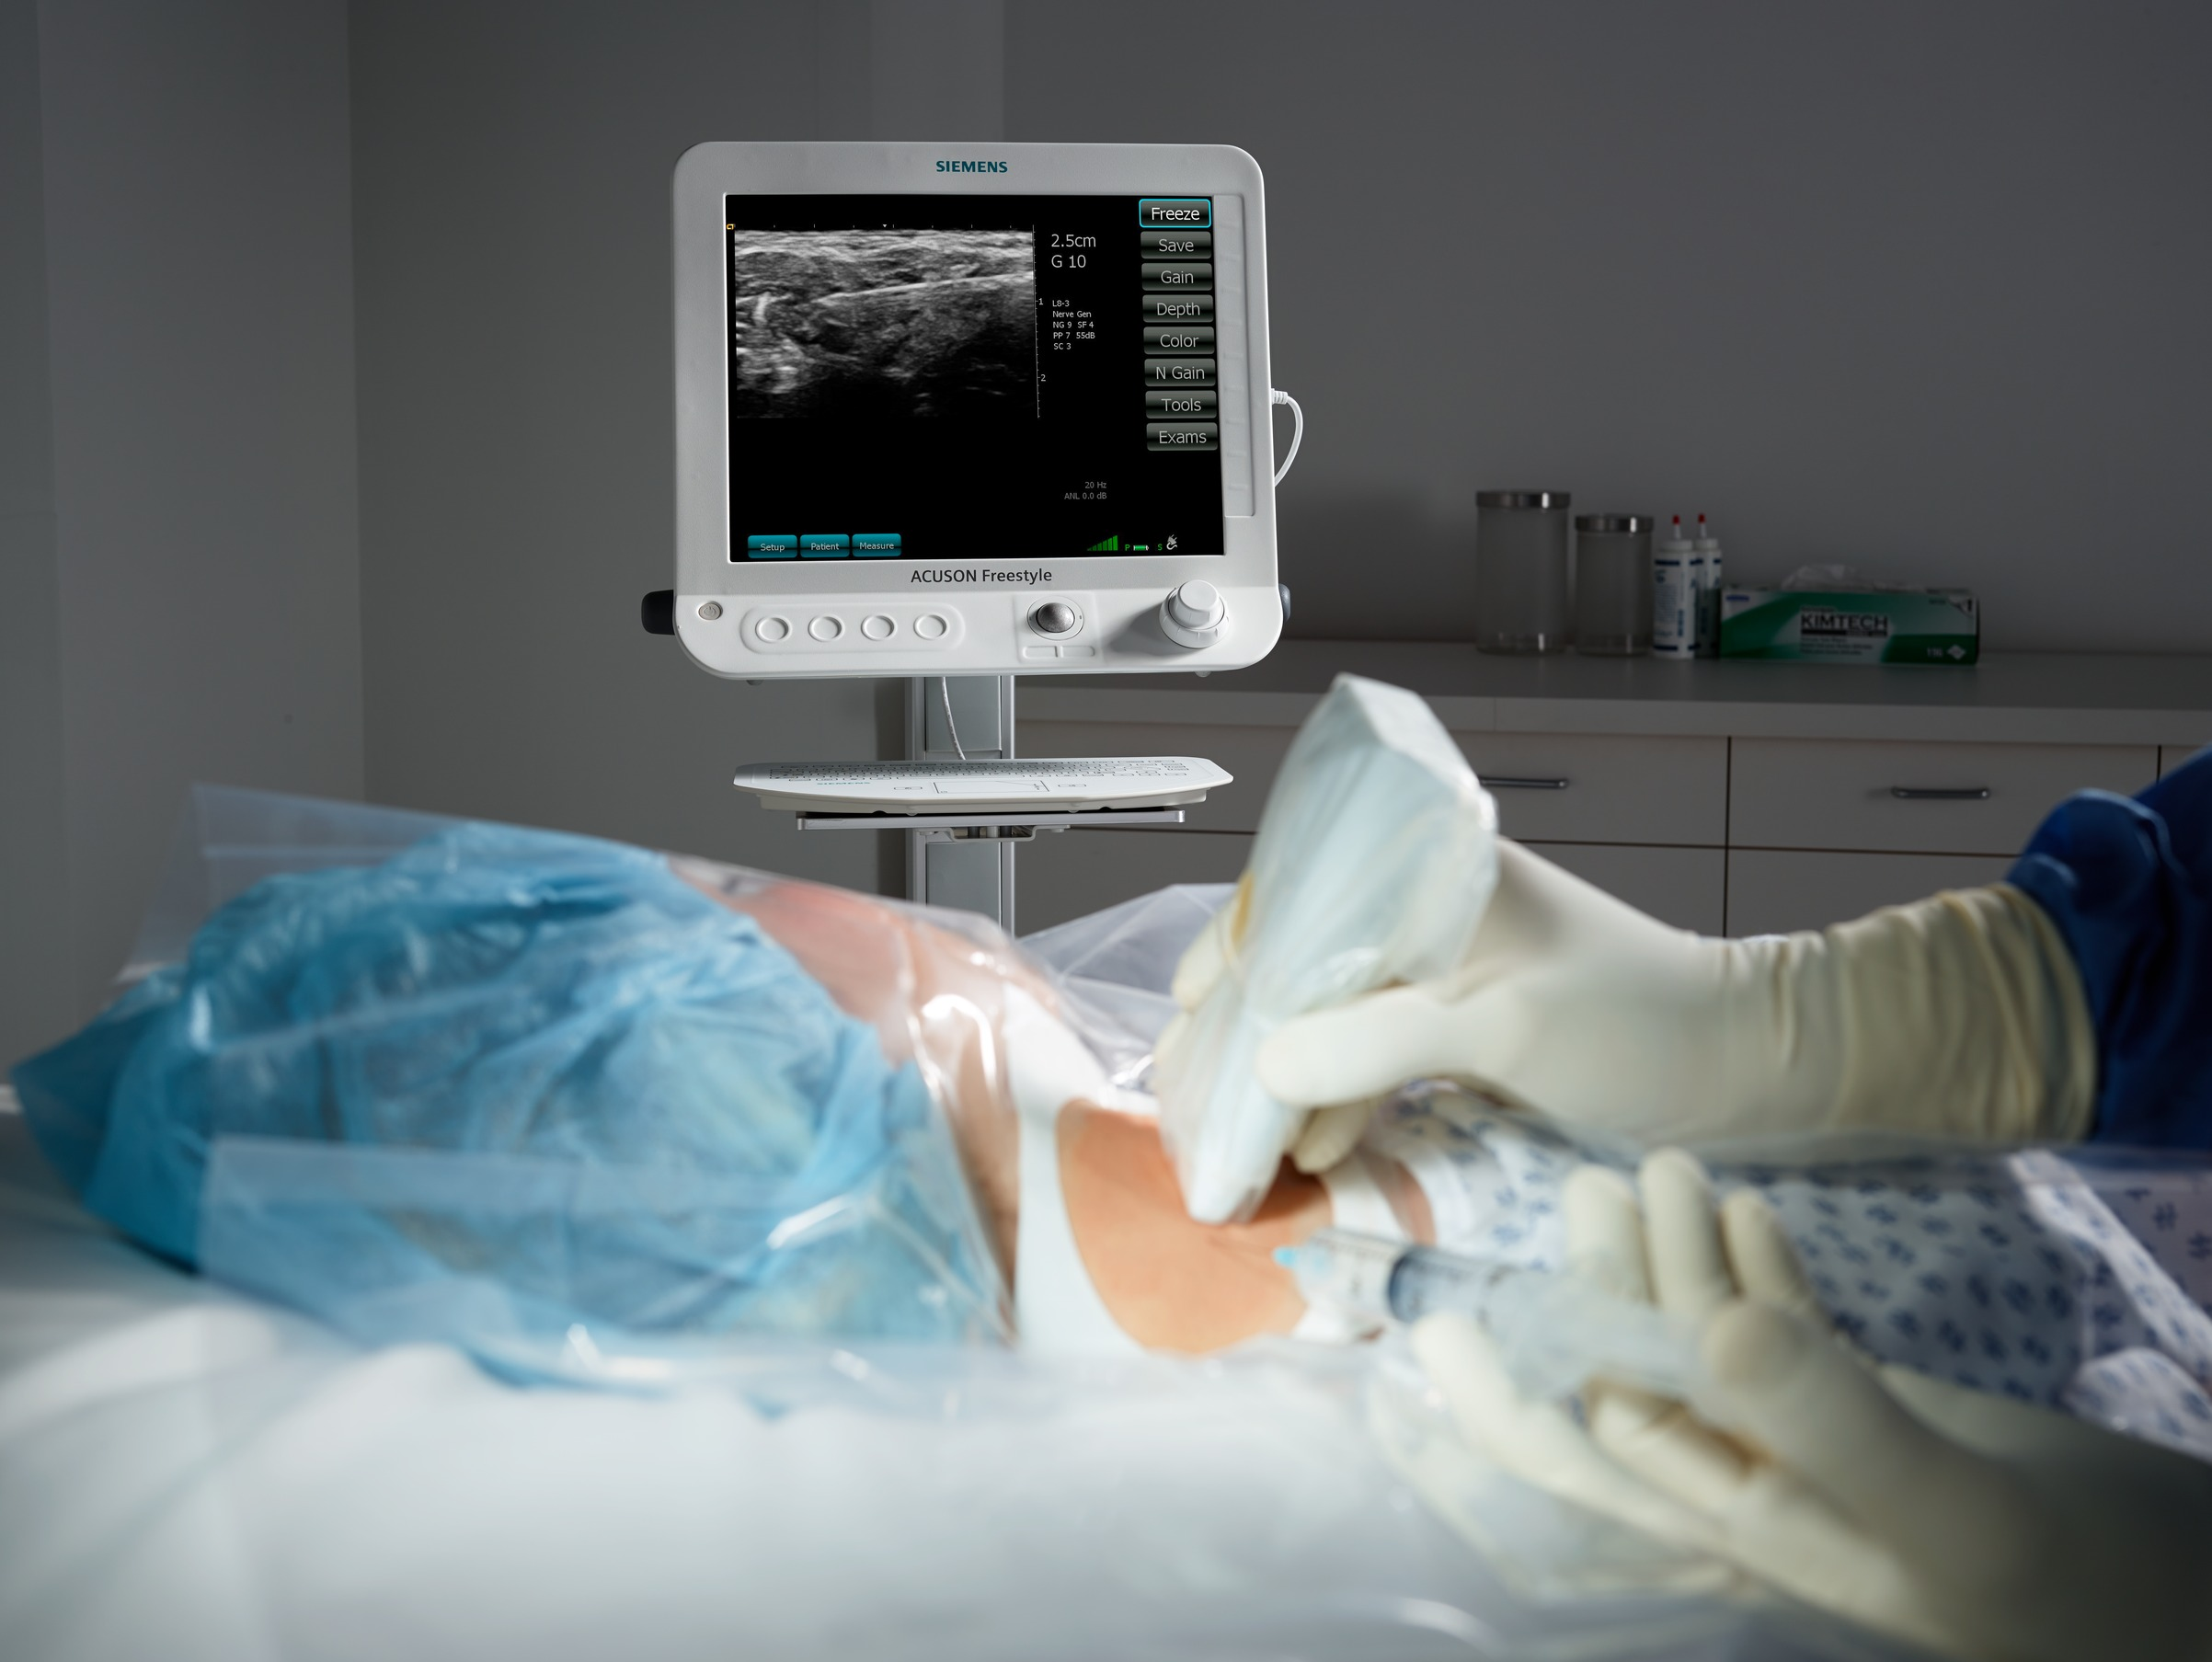
\includegraphics[width=0.9\columnwidth]{images/SH_US_39038_14.jpg}\\
            \begin{flushright}
                \tiny Source: Medical Imaging Systems~\cite{neumann18}
            \end{flushright}
        \end{figure}

    \end{columns}
\end{frame}


%%%%%%%%%%%%%%%%%%%%%%%%%%%%%%%%%%%%%%%%%%%%%%%%%%%%%%%%%%%%
\begin{frame}{Transducers \cont}

    \structure{Piezoelectric effect}
    \begin{itemize}
        \item Mechanical pressure (\emph{piezo} (gr.)) is converted to electric polarization\\
              $\rightarrow$ Electric voltage is generated (measurable using two electrodes)
              \vspace{.2cm}
        \item Electric field causes stretching of piezoelectric material\\
              $\rightarrow$ Can be used to generate sound waves
              \vspace{.2cm}
    \end{itemize}
    \def\svgwidth{.49\linewidth}\import{images/}{piezoelectric_effect.pdf_tex}%
    \begin{figure}
    \end{figure}
\end{frame}


%%%%%%%%%%%%%%%%%%%%%%%%%%%%%%%%%%%%%%%%%%%%%%%%%%%%%%%%%%%%%
%\begin{frame}{Transducers \cont}
%
%\structure{Transducer arrays}
%
%$\rightarrow$ Different geometries of transducer arrays are available
%\vspace{2cm}
%\begin{figure}
%\centering
%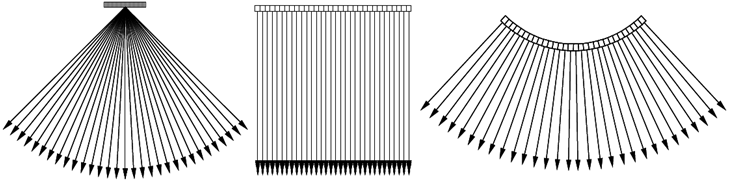
\includegraphics{images/transducer_arrays.png}\\
%{\Large Left to right: sector probe, linear array, curved array.}
%\end{figure}
%\end{frame}


%%%%%%%%%%%%%%%%%%%%%%%%%%%%%%%%%%%%%%%%%%%%%%%%%%%%%%%%%%%%
\begin{frame}{Spatial Resolution}

    \structure{Lateral} resolution
    \begin{itemize}
        \item Minimal distance perpendicular to US beam to distinguish two points
        \item Affected by beam width and depth of imaging
    \end{itemize}

    \vspace{.5cm}
    \structure{Axial} resolution
    \begin{itemize}
        \item Resolution in direction parallel to US beam
        \item Does \structure{not} change with depth
        \item Also known as longitudinal or azimuthal resolution
    \end{itemize}

    \vspace{-1cm}
    \flushright
    \def\svgwidth{.49\linewidth}
    \import{images/}{axial_vs_lateral.pdf_tex}

\end{frame}


%%%%%%%%%%%%%%%%%%%%%%%%%%%%%%%%%%%%%%%%%%%%%%%%%%%%%%%%%%%%
\begin{frame}{Spatial Resolution \cont}

    \structure{Axial} resolution \cont
    \begin{itemize}
        \item Shortest pulse: single wave
    \end{itemize}

    %\vspace{.5cm}
    \begin{figure}
        \def\svgwidth{\linewidth}
        \import{images/}{axial.pdf_tex}
    \end{figure}

\end{frame}


%%%%%%%%%%%%%%%%%%%%%%%%%%%%%%%%%%%%%%%%%%%%%%%%%%%%%%%%%%%%
\begin{frame}{Spatial Resolution \cont}

    \structure{Axial} resolution \cont
    \begin{itemize}
        \item Shortest pulse: single wave
    \end{itemize}

    %\vspace{.5cm}
    \begin{figure}
        \def\svgwidth{\linewidth}
        \import{images/}{axial2.pdf_tex}
    \end{figure}

    $\rightarrow$ Two \structure{distinguishable} echoes are generated only if $d > \lambda/2$.

    $\rightarrow$ Resolution decreases when $\lambda$ increases (frequency $f = c/\lambda $).
\end{frame}


%%%%%%%%%%%%%%%%%%%%%%%%%%%%%%%%%%%%%%%%%%%%%%%%%%%%%%%%%%%%
\begin{frame}{Spatial Resolution \cont}

    \structure{Frequency trade-off}
    \begin{itemize}
        \item Transducer frequency is directly related to resolution
              \begin{itemize}
                  \item High frequency $\rightarrow$ high resolution
                  \item Low frequency $\rightarrow$ low resolution
              \end{itemize}
              \vspace{.3cm}
        \item However, it is also directly related to attenuation
              \begin{itemize}
                  \item High frequency $\rightarrow$ high attenuation
                  \item Low frequency $\rightarrow$ low attenuation
              \end{itemize}
              \vspace{.3cm}
        \item High frequency $\rightarrow$ low penetration depth with high resolution
              \vspace{.3cm}
        \item Low frequency $\rightarrow$ deep penetration with low resolution
    \end{itemize}

\end{frame}


%%%%%%%%%%%%%%%%%%%%%%%%%%%%%%%%%%%%%%%%%%%%%%%%%%%%%%%%%%%%
\begin{frame}{Spatial Resolution \cont}

    \structure{Frequency trade-off \cont}
    \begin{columns}[b]
        \column{.45\textwidth}
        \begin{figure}
            \centering
            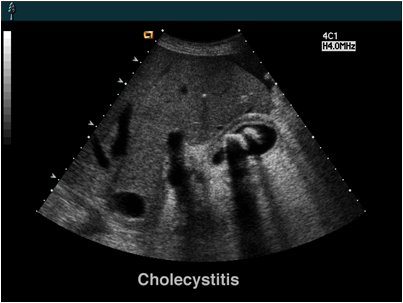
\includegraphics[width=.95\columnwidth]{images/frequency_example_4MHz.png}\\
            {\Large $f = 4$ MHz.}
        \end{figure}

        \column{.45\textwidth}
        \begin{figure}
            \centering
            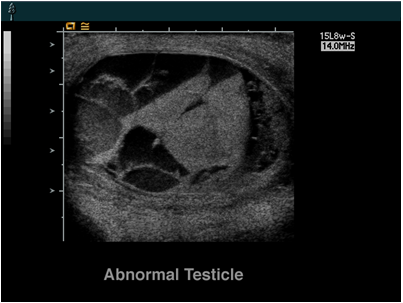
\includegraphics[width=.95\columnwidth]{images/frequency_example_14MHz.png}\\
            {\Large $f = 14$ MHz.}
        \end{figure}
    \end{columns}

\end{frame}


%%%%%%%%%%%%%%%%%%%%%%%%%%%%%%%%%%%%%%%%%%%%%%%%%%%%%%%%%%%%
%%%%%%%%%%%%%%%%%%%%%%%%%%%%%%%%%%%%%%%%%%%%%%%%%%%%%%%%%%%%
\section{Imaging Modes}
%%%%%%%%%%%%%%%%%%%%%%%%%%%%%%%%%%%%%%%%%%%%%%%%%%%%%%%%%%%%
%%%%%%%%%%%%%%%%%%%%%%%%%%%%%%%%%%%%%%%%%%%%%%%%%%%%%%%%%%%%


%%%%%%%%%%%%%%%%%%%%%%%%%%%%%%%%%%%%%%%%%%%%%%%%%%%%%%%%%%%%
\begin{frame}{Imaging Modes}

    \structure{Most common US imaging modes}
    \begin{itemize}
        \setlength\itemsep{0.3cm}
        \item A-mode
        \item B-mode
        \item M-mode
        \item Doppler mode
              \begin{itemize}
        \setlength\itemsep{0.1cm}
                  \item Pulse wave Doppler
                  \item Continuous wave Doppler
                  \item Spectral Doppler
                  \item Color Doppler
              \end{itemize}
    \end{itemize}

\end{frame}


%%%%%%%%%%%%%%%%%%%%%%%%%%%%%%%%%%%%%%%%%%%%%%%%%%%%%%%%%%%%
\begin{frame}{Imaging Modes \cont}

    \structure{A-mode}
    \begin{itemize}
        \item \textbf{A}mplitude-mode
        \item Single transducer scans on a line through the body (1D)
        \item Depth: time required for US beam to hit boundary and reflect signal
        \item Reflected signal strength can be measured (amplitude)
        \item Echoes are plotted on screen as function of depth
    \end{itemize}

    \vspace{1cm}
    $\rightarrow$ \structure{Simplest} scanning method.

\end{frame}


%%%%%%%%%%%%%%%%%%%%%%%%%%%%%%%%%%%%%%%%%%%%%%%%%%%%%%%%%%%%
\begin{frame}{Imaging Modes \cont}

    \structure{B-mode}
    \begin{itemize}
        \item \textbf{B}rightness-mode (or \structure{2D mode}): spatially encoded echo amplitude
        \item Time required for echo: position
        \item Amplitude: image \structure{brightness}
        \item Uses \structure{array} of transducers to generate 2D images
    \end{itemize}

    \vspace{.3cm}
    \begin{figure}
        \centering
        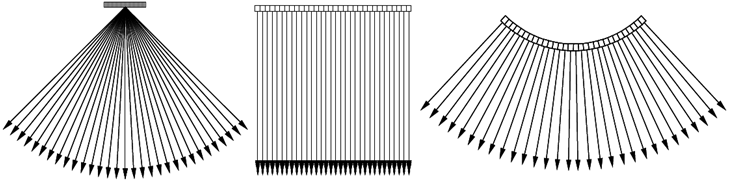
\includegraphics[width=.7\linewidth]{images/transducer_arrays.png}\\
        {\Large Left to right: sector probe, linear array, curved array.}
    \end{figure}


    $\rightarrow$ \structure{Most common} scanning method.

\end{frame}


%%%%%%%%%%%%%%%%%%%%%%%%%%%%%%%%%%%%%%%%%%%%%%%%%%%%%%%%%%%%
\begin{frame}{Imaging Modes \cont}

    \structure{B-mode \cont}
    \begin{columns}[b]
        \column{.45\textwidth}
        \begin{figure}
            \centering
            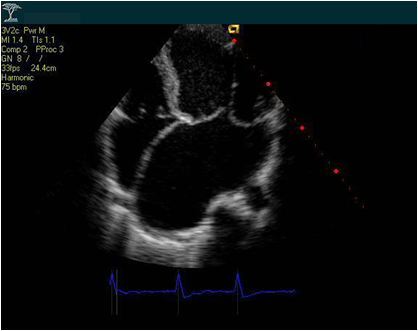
\includegraphics[width=.95\columnwidth]{images/b-mode_sector_probe.png}
            \caption{\normalsize Heart with enlarged atrium\newline (sector probe)}
        \end{figure}

        \column{.45\textwidth}
        \begin{figure}
            \centering
            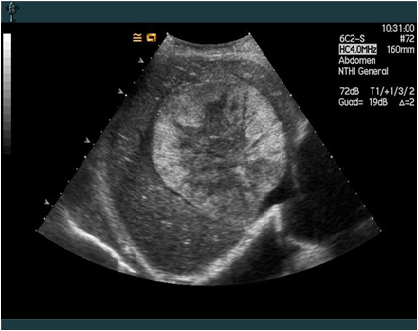
\includegraphics[width=.95\columnwidth]{images/b-mode_curved_array.png}
            \caption{\normalsize Liver with large tumor\newline (curved array)}
        \end{figure}
    \end{columns}

\end{frame}


%%%%%%%%%%%%%%%%%%%%%%%%%%%%%%%%%%%%%%%%%%%%%%%%%%%%%%%%%%%%
\begin{frame}{Imaging Modes \cont}

    \structure{B-mode \cont}

    \begin{figure}
        \centering
        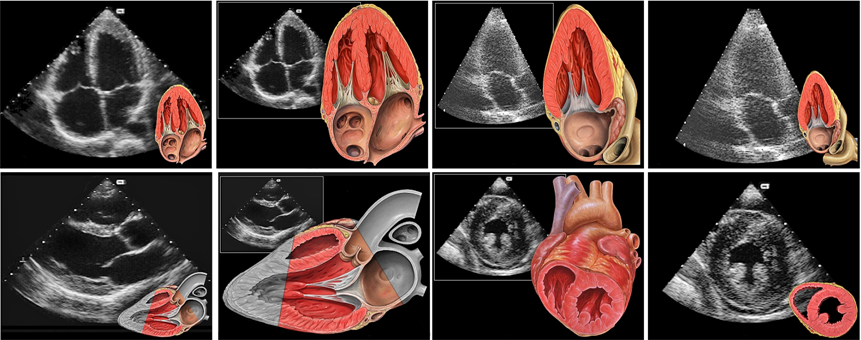
\includegraphics[width=.95\columnwidth]{images/b-mode_various.png}
        \caption{\normalsize Various views of the heart}
        \vspace{-0.7cm}
        \begin{flushright}
            \tiny Source: Patrick J. Lynch (\url{http://wikipedia.org/})
        \end{flushright}
    \end{figure}

\end{frame}


%%%%%%%%%%%%%%%%%%%%%%%%%%%%%%%%%%%%%%%%%%%%%%%%%%%%%%%%%%%%
\begin{frame}{Imaging Modes \cont}

    \structure{M-mode}
    \begin{itemize}
        \item \textbf{M}otion-mode
        \item Pulses are emitted in quick succession (same probe position)
        \item Either an A-mode or a B-mode image is taken each time
        \item Time-dependent organ movement relative to the probe can be measured\\
              $\rightarrow$ velocity of specific organ structures
    \end{itemize}

    \vspace{1cm}
    $\rightarrow$ Example: Cardiac (echocardiography) wall movement analysis.

\end{frame}


%%%%%%%%%%%%%%%%%%%%%%%%%%%%%%%%%%%%%%%%%%%%%%%%%%%%%%%%%%%%
\begin{frame}{Imaging Modes \cont}

    \structure{M-mode \cont}

    \begin{figure}
        \centering
        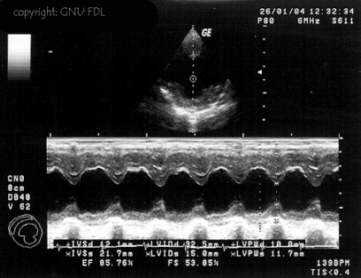
\includegraphics[height=0.7\textheight]{images/m-mode_example.png}
        \caption{\normalsize Combined B- and M-mode visualization of dog heart}
        \vspace{-0.5cm}
        \begin{flushright}
            \tiny  Source: \url{http://wikipedia.org/}
        \end{flushright}
    \end{figure}
\end{frame}


%%%%%%%%%%%%%%%%%%%%%%%%%%%%%%%%%%%%%%%%%%%%%%%%%%%%%%%%%%%%
\begin{frame}{Imaging Modes \cont}

    \structure{Doppler ultrasonography}
    \vspace{0.3cm}
    \begin{itemize}
        \setlength\itemsep{0.3cm}
        \item Enables visualization of blood \structure{flow} (velocity)
        \item \structure{Continuous wave} (CW) Doppler\\
              $\rightarrow$ Half of transducer array emits, half detects pulses (simultaneously)\\
              $\rightarrow$ No distance information
        \item \structure{Pulsed Wave} (PW) Doppler\\
              $\rightarrow$ Pulse-based\\
              $\rightarrow$ Distance information is obtained (time-gating)
    \end{itemize}

    \vspace{1cm}
    $\rightarrow$ Makes use of the \structure{Doppler effect}.
\end{frame}


%%%%%%%%%%%%%%%%%%%%%%%%%%%%%%%%%%%%%%%%%%%%%%%%%%%%%%%%%%%%
\begin{frame}{Imaging Modes \cont}

    \structure{Doppler ultrasonography \cont{} -- Doppler effect}
    \begin{itemize}
        \setlength\itemsep{0.3cm}
        \item Change in wave frequency by relative movement between \structure{source} and \structure{observer}
        \item Characteristic frequency shifts appear $\rightarrow$ proportional to velocity
        \item Named after Christian Johann Doppler ($\ast$1803, \textdagger{} 1853)
        \item Examples
              \begin{itemize}
                  \item Siren of ambulance
                  \item Astronomical red-shift
                  \item Blood flow
              \end{itemize}
    \end{itemize}

\end{frame}


%%%%%%%%%%%%%%%%%%%%%%%%%%%%%%%%%%%%%%%%%%%%%%%%%%%%%%%%%%%%
\begin{frame}{Imaging Modes \cont}

    \structure{Doppler ultrasonography \cont}
    \begin{itemize}
        \item Doppler effect in US \structure{blood flow} imaging
              \begin{itemize}
                  \item Source: \structure{Moving} blood cells (through \structure{scattering} of US wave)
                  \item Observer: US transducer
                  \item Doppler angle $\theta$ (between blood and sound direction) $\rightarrow$ the smaller the better
              \end{itemize}
    \end{itemize}

    \begin{figure}
        \def\svgwidth{.9\linewidth}
        \import{images/}{doppler_blood_flow.pdf_tex}
    \end{figure}

\end{frame}


%%%%%%%%%%%%%%%%%%%%%%%%%%%%%%%%%%%%%%%%%%%%%%%%%%%%%%%%%%%%
\begin{frame}{Imaging Modes \cont}

    \structure{Doppler ultrasonography \cont}
    \vspace{0.3cm}
    \begin{itemize}
        \setlength\itemsep{0.3cm}
        \item \structure{Spectral} Doppler\\
              $\rightarrow$ Visualize spectrum of blood speeds
        \item \structure{Color} Doppler\\
              $\rightarrow$ Color-coded overlay on top of B-mode image
    \end{itemize}

    %\vspace{1cm}
    %$\rightarrow$ The term \structure{Doppler ultrasonography} applies for both CW and PW doppler.

\end{frame}


%%%%%%%%%%%%%%%%%%%%%%%%%%%%%%%%%%%%%%%%%%%%%%%%%%%%%%%%%%%%
\begin{frame}{Imaging Modes \cont}

    \structure{Doppler ultrasonography \cont}
    \begin{figure}
        \centering
        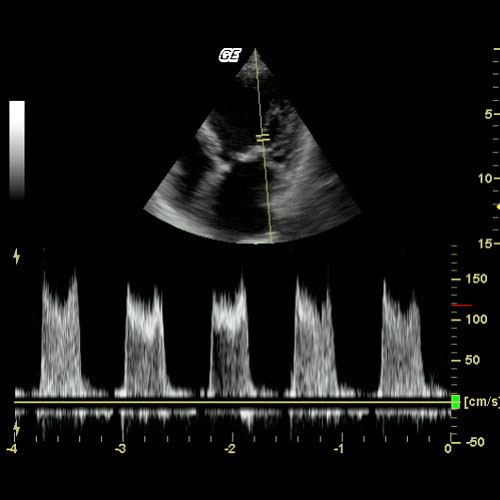
\includegraphics[height=0.7\textheight]{images/spectral_doppler_ge.jpg}
        \caption{\normalsize Spectral doppler. }
        \begin{flushright}
            \tiny Source: \url{http://gehealthcare.com/}
        \end{flushright}
    \end{figure}
\end{frame}


%%%%%%%%%%%%%%%%%%%%%%%%%%%%%%%%%%%%%%%%%%%%%%%%%%%%%%%%%%%%
\begin{frame}{Imaging Modes \cont}

    \structure{Doppler ultrasonography \cont}
    \begin{figure}
        \begin{center}
            \animategraphics[height=0.7\textheight,autoplay,loop]{3}{images/gif/doppler_mitral_valve-}{0}{9}

            \caption{Mitral valve insufficiency (dog heart), color doppler}
            \begin{flushright}
                \tiny Source: \url{http://wikipedia.org/}
            \end{flushright}
        \end{center}
    \end{figure}
\end{frame}


%%%%%%%%%%%%%%%%%%%%%%%%%%%%%%%%%%%%%%%%%%%%%%%%%%%%%%%%%%%%
\begin{frame}{Imaging Modes \cont}

    \structure{Dimensionality of acquired images}
    \begin{itemize}
        \setlength\itemsep{0.1cm}
        \item 1D $\rightarrow$ A- or M-mode
        \item 2D $\rightarrow$ many B-mode scan lines (e.g.~linear/curved transducer array)
        \item 3D $\rightarrow$ several 2D images at different angles combined into single volume
        \item 4D $\rightarrow$ 3D + time
    \end{itemize}

\end{frame}


%%%%%%%%%%%%%%%%%%%%%%%%%%%%%%%%%%%%%%%%%%%%%%%%%%%%%%%%%%%%
%%%%%%%%%%%%%%%%%%%%%%%%%%%%%%%%%%%%%%%%%%%%%%%%%%%%%%%%%%%%
\section{Safety in US Imaging}
%%%%%%%%%%%%%%%%%%%%%%%%%%%%%%%%%%%%%%%%%%%%%%%%%%%%%%%%%%%%
%%%%%%%%%%%%%%%%%%%%%%%%%%%%%%%%%%%%%%%%%%%%%%%%%%%%%%%%%%%%


%%%%%%%%%%%%%%%%%%%%%%%%%%%%%%%%%%%%%%%%%%%%%%%%%%%%%%%%%%%%
\begin{frame}{Safety in US Imaging}

    US waves are \structure{not ionizing}, however they can harm the body \dots
    \begin{itemize}
        \item \dots through heating\\
              \hspace{1cm}{$\rightarrow$ locally, proportional to absorbed acoustic intensity ($J$)}
        \item \dots through cavitation\\
              \hspace{1cm}{$\rightarrow$ emerging gas bubbles in low pressure phase of sound wave}\\
              \hspace{1cm}{$\rightarrow$ collapse at high pressure phase}
    \end{itemize}
    \vspace{.5cm}
    $\rightarrow$ Acoustic intensities for medical diagnostics rather low\\
    $\rightarrow$ \structure{harmless}, it is even used during pregnancy

    \structure{Therapeutical use of ultrasound}
    \begin{itemize}
        \item Break up gallstones and kidney stones
        \item Heat and destroy diseased or cancerous tissue
    \end{itemize}
\end{frame}


\end{document}
